\documentclass{article}

\usepackage{graphicx}
\graphicspath{ {./images/} }

\usepackage{tikz}
\def\firstcircle{(90:1.5cm) circle (2cm)}
\def\secondcircle{(210:1.5cm) circle (2cm)}
\def\thirdcircle{(330:1.5cm) circle (2cm)}
\begin{document}
        
%Header
\begin{flushleft}
    Evan Wilcox\\
    CS1200 Fall 2018\\
    Homework 5\\
    Due: Wednesday 11/07/18
\end{flushleft}
        
%Problems
\begin{enumerate}

    %1
    \item Assuming P and Q are defined for the same universe use truth
    trees to determine whether the argument is valid. If it is not valid construct a counterexample.

    %2
    \item Draw a Venn diagram to show the relationships among the sets.
    
    %3
    \item Write a Python program to verify your answers.
    
    %4
    \item  Simplify the expression $(A \cup ((B \cap C)' \cup (A' \cap C')')')'$using the laws of Boolean algebra.

    %5
    \item Write down the set $\{x, y\} \times \{f, h\} \times \{9, 3, 6\}$.
    
    %6
    \item
    \begin{enumerate}
        
        %a
        \item List all the elements of $2^{\{0,1,2\}}$ and $2^{\{a,b,c,d\}}$.
    
        $$\{\{\}, \{0\}, \{1\}, \{2\}, \{0, 1\}, \{0, 2\}, \{1, 2\}, \{0, 1, 2\}\}$$
        $$\{\{\}, \{a\}, \{b\}, \{c\}, \{d\}, \{a, b\}, \{a, c\}, \{a, d\}\},\{b, c\}, $$
        $$\{b, d\},\{c, d\}, \{a, b, c\}, \{a, b, d\}, \{a, c, d\}, \{b, c, d\}, \{a, b, c, d\}\}$$
        
        %b
        \item Write a Python program to verify your answers in (a).
    
    \end{enumerate}

    %7
    \item Draw a Venn diagram of $(A\#B) \cap (B\#C)$.
    \begin{center}
    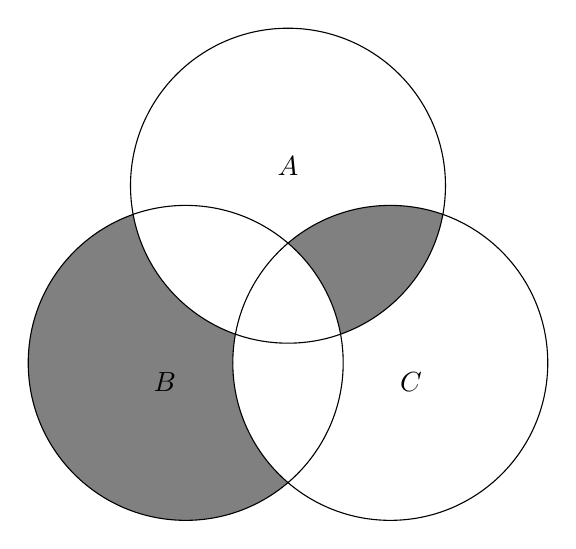
\begin{tikzpicture}
        \begin{scope}
            \clip \firstcircle;
            \fill[gray] \thirdcircle;
        \end{scope}
        
        \begin{scope}
            \fill[gray] \secondcircle;
        \end{scope}

        \begin{scope}
            \clip \secondcircle;
            \fill[white] \thirdcircle;
        \end{scope}

        \begin{scope}
            \clip \secondcircle;
            \fill[white] \firstcircle;
        \end{scope}
        
        \draw \firstcircle node[text=black,above] {$A$};
        \draw \secondcircle node [text=black,below left] {$B$};
        \draw \thirdcircle node [text=black,below right] {$C$};
    \end{tikzpicture}
    \end{center}

    %8
    \item Assuming P, Q and R are defined for the same universe
    use truth trees to decide if the following argument is valid. If it is
    not valid show all the counterexamples that can be found using the truth
    tree.






\end{enumerate}

\end{document}